\documentclass[a4paper,12pt]{book}
%\usepackage{mathpazo}
\usepackage{amsmath} % จะใช้ package ของ math อื่นใด ให้เรียกก่อน fontspec
\usepackage{amssymb} % จะใช้ package ของ math อื่นใด ให้เรียกก่อน fontspec
\usepackage{amsfonts} % จะใช้ package ของ math อื่นใด ให้เรียกก่อน fontspec
\usepackage{mathspec} % เรียกใช้แค่นี้มีค่า = \usepackage[no-math]{fontspec}\usepackage{mathspec}
\usepackage{xunicode,xltxtra}
\XeTeXlinebreaklocale "th"
\XeTeXlinebreakskip = 0pt plus 1pt %
\defaultfontfeatures{Scale=1.23}
\renewcommand{\baselinestretch}{1.2}
\setmainfont{TH Sarabun New}
\newfontfamily\kodchasal{TH Kodchasal} % ตั้งชื่อฟอนต์ใหม่เพื่อให้ง่ายต่อการใช้งาน เผื่อว่าในเอกสารต้องการให้มีหลายฟอนต์ เวลาใช้ก็ {\examplefont ข้อความต่าง ๆ}
\newfontfamily\niramit{TH Niramit AS}
\usepackage{xcolor}
\definecolor{MyColor}{rgb}{0.3,0.4,0.5} % กำหนดสี และชื่อที่จะใช้เรียกสีโดย xcolor
\everymath{\displaystyle} % บังคับให้ทุกสมการเป็น displaystyle
\usepackage{tabls}
\usepackage{graphicx}
\usepackage{tabularx}
\usepackage{booktabs}
\usepackage{longtable}
\usepackage{wrapfig} %ตัวหนังสือล้อมรอบรูปหรือตารางได้ (wrapfigure,wraptable) *** ไม่สามารถอยู่ในพวก enumerate ได้
\usepackage[Glenn]{fncychap}
\usepackage{sectsty,ulem}
\allsectionsfont{\ulemheading{\uline}}
\makeatletter
\def\@seccntformat#1{\csname the#1\endcsname)\quad}
\makeatother
\usepackage{cellspace}
\usepackage[usenames,dvipsnames]{pstricks} 
\usepackage{epsfig} 
\usepackage{pst-grad} % For gradients
\usepackage{pst-plot} % For axes 
\usepackage{makecell}
\usepackage{fancyhdr}
\usepackage{lastpage}
\usepackage{fancybox}
\usepackage{multirow}
\usepackage{calc}
% ระยะช่องว่างหน้า+หลังเลขหรืออักษรในสมการ หน่วยเป็น mmu , 1 mmu = 1mu/1000 , 18mu = 1 em ,default = 500 mmu = 1/36 em 
% ตัวไหนจะให้มีระยะพิเศษก็ใส่ " นำหน้า เช่น $ x^{"2} หรือใส่ทีละคำให้ใส่เป็น $ x^{\"3yz"} $
% \setminwhitespace[XXXX] 
\setminwhitespace[3000] 

% เลือก Math Font ต่าง ๆ นา ๆ
%\setmathsfont(Digits,Latin){Asana Math}
%\setmathsfont(Digits,Latin){jsMath-cmr10}
%\setmathsfont(Digits,Latin){Kerkis}
%\setmathsfont(Digits,Latin){Neo Euler}
%\setmathsfont(Digits,Latin){Fontin}
%\setmathsfont(Digits,Latin){Plakken}
%\setmathsfont(Digits,Latin){DejaVu Serif}
%\setmathsfont(Digits,Latin){STIXGeneral}
%\setmathsfont(Digits,Latin){CMU Bright}
%\setmathsfont(Digits,Latin){Iwona Light}
%\setmathsfont(Digits,Latin,Greek)[Numbers={Lining,Proportional}]{Iwona Light}
%\setmathsfont(Digits,Latin,Greek){TH Sarabun New}
%\setmathsfont(Digits,Latin,Greek){Mathmos Original}
% ใช้ฟอนต์ OTF ในเอกสารแต่ MATH ใช้ฟอนต์ Math
%\usepackage[no-math]{fontspec}

% ใช้ฟอนต์ OTF ในเอกสารและ MATH ใช้ฟอนต์ OTF
%\usepackage[no-math]{fontspec}
%\usepackage{mathspec}
%\setmainfont{TH Sarabun New}
%\setallmainfonts(Digits,Latin,Greek){TH Sarabun New}
\setallmainfonts(Digits,Latin,Greek){TH Sarabun New}

% \setmathrm จะเปลี่ยนฟอนต์เฉพาะที่อยู่ในคำสั่ง \mathrm{.....} เท่านั้น
%\setmathrm{TH Sarabun New}
%\setmathsfont(Digits,Latin,Greek){TH Sarabun New}
%\setmathfont(Digits,Latin,Greek){TH Sarabun New}

\pagestyle{fancy}
\fancyhead[L]{ติวสบายฟิสิกส์}
\fancyhead[R]{www.pec9.com}
% ------- เอารูปวางตรงไหนก็ได้ในเอกสาร ---------
% ------- ใช้ทำเส้นข้างร่วมกับ fancyhdr ----------
\usepackage{eso-pic,picture}
\usepackage{exsheets} % Create ex­er­cise sheets and ex­ams
\setlist[enumerate,1]{leftmargin=*,resume} % ตั้งให้ enumerate level 1 ไม่ indent และต่อข้ออัตโนมัติ โดยไม่ต้องใช้ counter


\begin{document}
\begin{enumerate}
\item 	\begin{ljrp} 
		 	ระยะทางและการกระจัดของการเคลื่อนที่ต่อไปนี้ มีขนาดเท่ากับกี่เมตรตามลําดับ
			\begin{4c}
				{das}{sada}{dsad}{sadd}
			\end{4c}
		\end{ljrp}
		\begin{rp}{test_env.eps}\end{rp}
\end{enumerate}
\begin{enumerate}
\item 	\begin{ljrp} 
		 	ระยะทางและการกระจัดของการเคลื่อนที่ต่อไปนี้ มีขนาดเท่ากับกี่เมตรตามลําดับ
			\begin{2c}
				{das}{sada}{dsad}{sadd}
			\end{2c}
		\end{ljrp}
		\begin{rp}{test_env.eps}\end{rp}
\end{enumerate}
\begin{enumerate}
\item 	\begin{ljrp} 
		 	ระยะทางและการกระจัดของการเคลื่อนที่ต่อไปนี้ มีขนาดเท่ากับกี่เมตรตามลําดับ
			\begin{1c}
				{das}{sada}{dsad}{sadd}
			\end{1c}
		\end{ljrp}
		\begin{rp}{test_env.eps}\end{rp}
\end{enumerate}
\begin{enumerate}
\item 	\begin{ljrp} 
		 	ระยะทางและการกระจัดของการเคลื่อนที่ต่อไปนี้ มีขนาดเท่ากับกี่เมตรตามลําดับ
		\end{ljrp}
		\begin{rp}{test_env.eps}\end{rp}
		\begin{4c}
			{das}{sada}{dsad}{sadd}
		\end{4c}
\end{enumerate}
\begin{enumerate}
\item 	\begin{ljrp} 
		 	ระยะทางและการกระจัดของการเคลื่อนที่ต่อไปนี้ มีขนาดเท่ากับกี่เมตรตามลําดับ
		\end{ljrp}
		\begin{rp}{test_env.eps}\end{rp}
		\begin{2c}
			{das}{sada}{dsad}{sadd}
		\end{2c}
\end{enumerate}
\begin{enumerate}
\item 	\begin{ljrp} 
		 	ระยะทางและการกระจัดของการเคลื่อนที่ต่อไปนี้ มีขนาดเท่ากับกี่เมตรตามลําดับ
		\end{ljrp}
		\begin{rp}{test_env.eps}\end{rp}
		\begin{1c}
			{das}{sada}{dsad}{sadd}
		\end{1c}
\end{enumerate}
\begin{enumerate}
\item	\begin{lp}{test_env.eps}\end{lp}
		\begin{rjlp}
			ระยะทางและการกระจัดของการเคลื่อนที่ต่อไปนี้ มีขนาดเท่ากับกี่เมตรตามลําดับ
		\end{rjlp}
		\begin{4c}
			{das}{sada}{dsad}{sadd}
		\end{4c}
\end{enumerate}
\begin{enumerate}
\item	\begin{lp}{test_env.eps}\end{lp}
		\begin{rjlp}
			ระยะทางและการกระจัดของการเคลื่อนที่ต่อไปนี้ มีขนาดเท่ากับกี่เมตรตามลําดับ
		\end{rjlp}
		\begin{2c}
			{das}{sada}{dsad}{sadd}
		\end{2c}
\end{enumerate}
\begin{enumerate}
\item	\begin{lp}{test_env.eps}\end{lp}
		\begin{rjlp}
			ระยะทางและการกระจัดของการเคลื่อนที่ต่อไปนี้ มีขนาดเท่ากับกี่เมตรตามลําดับ
		\end{rjlp}
		\vspace{-25pt}
		\begin{1c}
			{das}{sada}{dsad}{sadd}
		\end{1c}
\end{enumerate}

\begin{enumerate}
	\item 	\begin{minipage}[t]{.65\textwidth}
				ระยะทางและการกระจัดของการเคลื่อนที่ต่อไปนี้ มีขนาดเท่ากับกี่เมตรตามลําดับ
				\begin{multienumerate}
					\setlength{\labelwidth}{8pt}
					\mitemxxxx{x1}{x2}{x3}{x4}
				\end{multienumerate}
			\end{minipage}
			\hfill
			\begin{adjustbox}{valign=t} 
  				\begin{minipage}[t]{0.3\linewidth} 
				  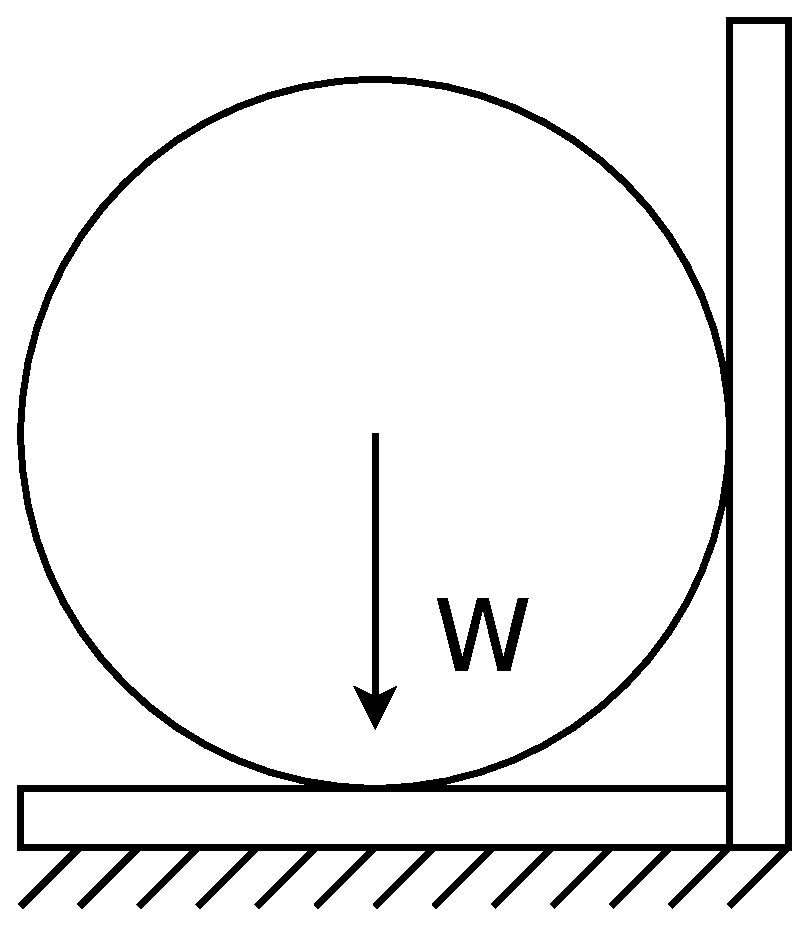
\includegraphics[width=\textwidth]{test_env.eps} 
				\end{minipage} 	
			\end{adjustbox} 
	\item 	\begin{minipage}[t]{.65\textwidth}
				ระยะทางและการกระจัดของการเคลื่อนที่ต่อไปนี้ มีขนาดเท่ากับกี่เมตรตามลําดับ
				\begin{multienumerate}
					\setlength{\labelwidth}{8pt}
					\mitemxx{x1}{x2}
					\mitemxx{x3}{x4}
				\end{multienumerate}
			\end{minipage}
			\hfill
			\begin{adjustbox}{valign=t} 
  				\begin{minipage}[t]{0.3\linewidth} 
				  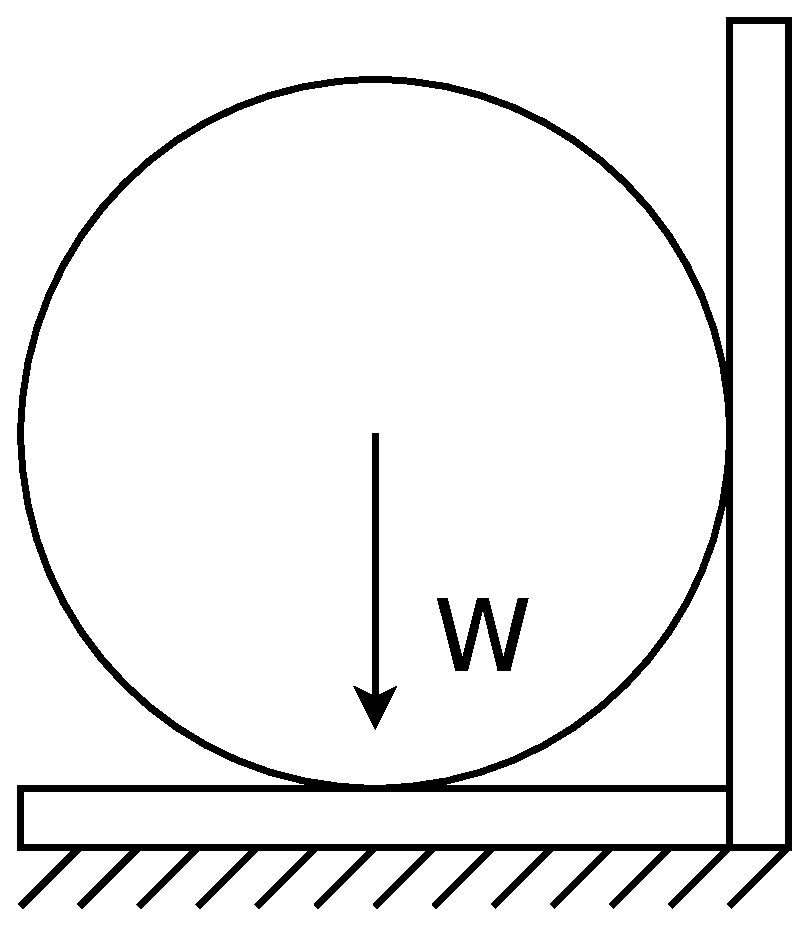
\includegraphics[width=\textwidth]{test_env.eps} 
				\end{minipage} 	
			\end{adjustbox} 
	\item 	\begin{minipage}[t]{.65\textwidth}
				ระยะทาง และ การกระจัดของการเคลื่อนที่ต่อไปนี้ มีขนาดเท่ากับกี่เมตรตามลําดับ
				\begin{multienumerate}
					%\vspace{-5pt}
					\setlength{\labelwidth}{8pt}
					\setlength{\itemsep}{0pt}
					\mitemxx{x1}{x2}
					\mitemxx{x3}{x4}
				\end{multienumerate}
			\end{minipage}
			\hfill
			\begin{adjustbox}{valign=t} 
  				\begin{minipage}[t]{0.3\linewidth} 
				  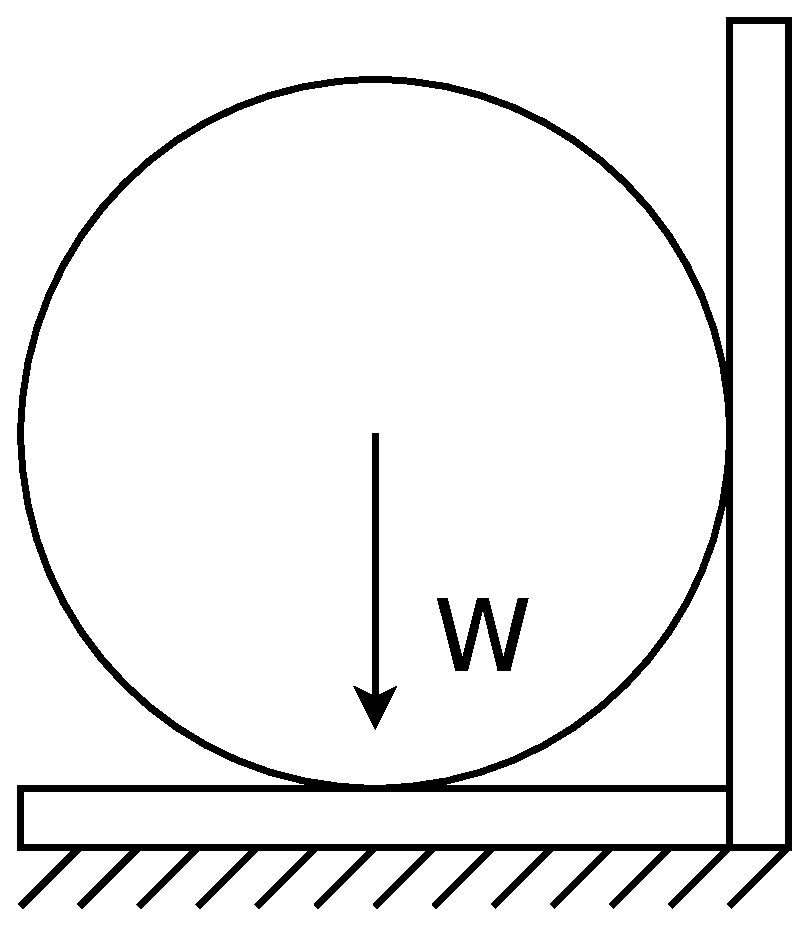
\includegraphics[width=\textwidth]{test_env.eps} 
				\end{minipage} 	
			\end{adjustbox} 
	\item 	\begin{minipage}[t]{.65\textwidth}
				ระยะทางและการกระจัดของการเคลื่อนที่ต่อไปนี้ มีขนาดเท่ากับกี่เมตรตามลําดับ
				\begin{multienumerate}
					\setlength{\labelwidth}{8pt}
					\setlength{\itemsep}{0pt}
					\mitemx{x1}
					\mitemx{x2}
					\mitemx{x3}
					\mitemx{x4}
				\end{multienumerate}
			\end{minipage}
			\hfill
			\begin{adjustbox}{valign=t} 
  				\begin{minipage}[t]{0.3\linewidth} 
				  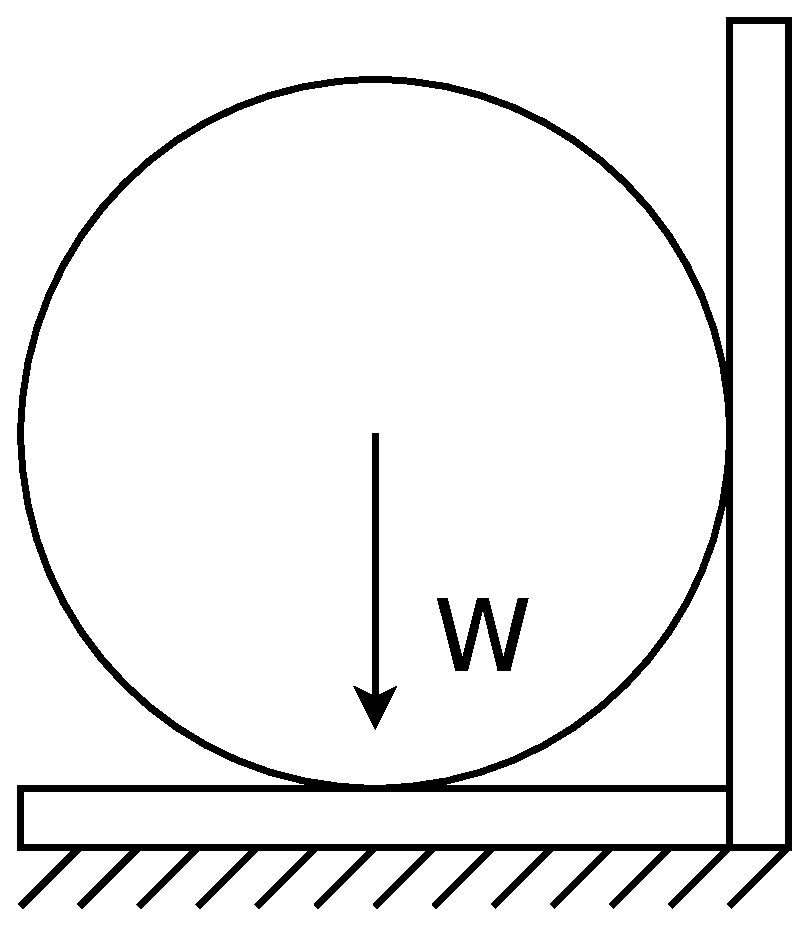
\includegraphics[width=\textwidth]{test_env.eps} 
				\end{minipage} 	
			\end{adjustbox} 
	\item 	\begin{minipage}[t]{.65\textwidth}
				ระยะทางและการกระจัดของการเคลื่อนที่ต่อไปนี้ มีขนาดเท่ากับกี่เมตรตามลําดับ
				\begin{multienumerate}
					\mitemx{x1}
					\mitemx{x2}
					\mitemx{x3}
					\mitemx{x4}
				\end{multienumerate}
			\end{minipage}
			\hfill
			\begin{adjustbox}{valign=t} 
  				\begin{minipage}[t]{0.3\linewidth} 
				  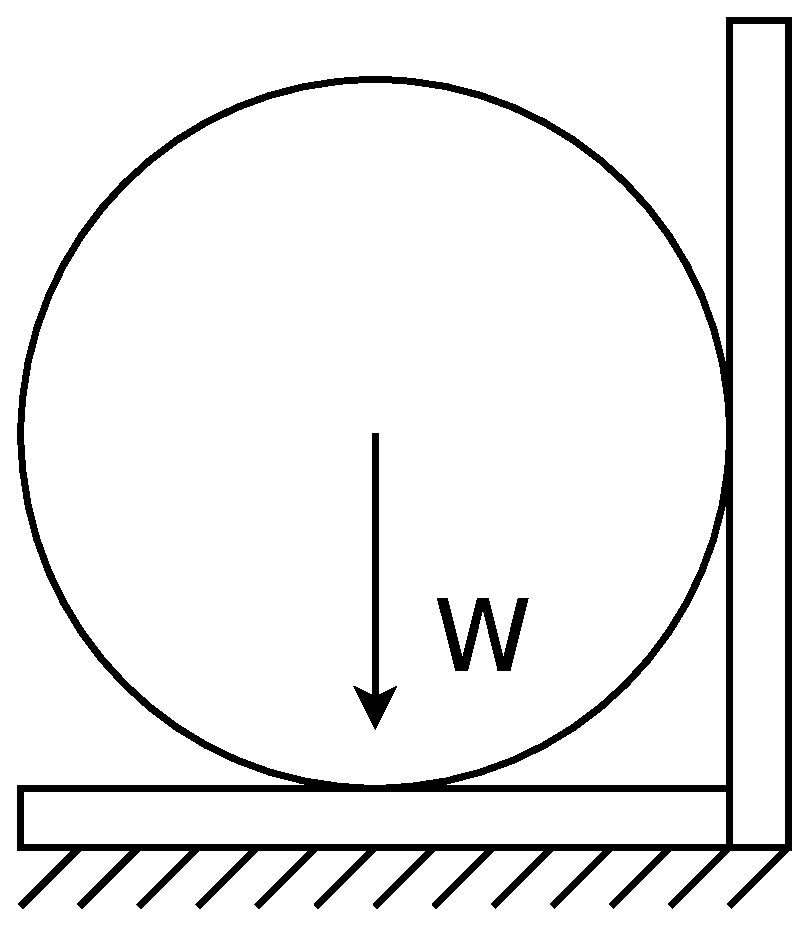
\includegraphics[width=\textwidth]{test_env.eps} 
				\end{minipage} 	
			\end{adjustbox} 
\end{enumerate}

\end{document}
